\subsection{Chorregent in schwieriger Zeit}
\hypertarget{RefHeadingToc100333735}{}Am 25.1.1940 starb der erst 36
Jahre alte Chorregent und Gemeindesekretär Albert Schroll, der 10 Jahre
lang in Ruhmannsfelden wirkte. \footnote{Korrespondenz Nr. 90, Brief
von Pfarramt Kollnburg an Josef Friedrich, 13.1.2005} Er erkrankte
schon 1939, sodass der Lehrer Ertl für Schroll als Klavierbegleiter bei
einem Singspiel einspringen musste. \footnote{Interview Nr. 16, Maria
Freisinger, 25.8.2004; Absatz 44} August Högn vertrat Schroll als
Chorregent und Organist während seiner Krankheit und nach dessen Tod
übernahm er seine Stelle \footnote{Interview Nr. 2, Barbara Essigmann,
27.12.2002, Absatz 6} aushilfsweise, wie es den Chorabrechnungen zu
entnehmen ist. \footnote{Dokument Nr. 136, Chorabrechnung Beerdigungen
und Trauungen, 3. Quartal 1952; Dokument Nr. 137, Chorabrechnung Ämter
und Messen, 3. Quartal 1952} Der 61-jährige und daher nicht mehr
wehrfähige Högn blieb aber Chorregent und Organist während des gesamten
2. Weltkriegs, da aufgrund der Kriegssituation kein hauptamtlicher
Kirchenmusiker als Nachfolger für Schroll verfügbar war. Nach dem Krieg
wurde Högn infolge der Entnazifizierung vom Schuldienst suspendiert und
dann in den Ruhestand versetzt, sodass der Weiterführung der
Chorregententätigkeit durch Högn in Form der Unvereinbarkeit von Schul-
und Kirchendienst nichts mehr im Wege stand. Zu Beginn von Högns
dritter Chorregentenzeit kehrte man gezwungenermaßen zur gewohnten
Praxis zurück, bei Beerdigungen den Unterricht ausfallen zu
lassen. \footnote{Interview Nr. 16, Maria Freisinger, 25.8.2004, Absatz
6; Interview Nr. 6, Wilhelm Ederer, 2.1.2003, Absatz 6} Diese in der
Weimarer Republik geduldete Regelung wurde von den Behörden des
religionsfeindlichen NS-Regimes bald unterbunden. Josef Brunner – er
war zu jung für den Kriegseinsatz \footnote{Interview Nr. 8, Josef
Brunner, 3.1.2003, Absatz 2} – und eine Mallersdorfer Schwester, die an
der Kinderbewahranstalt arbeitete, übernahmen deshalb den
Organistendienst bei Beerdigungen an Stelle von August Högn.\footnote{
Interview Nr. 16, Maria Freisinger, 25.8.2004, Absatz 6}

\begin{center}
\begin{minipage}{5.593cm}
\begin{flushleft}
\tablefirsthead{}
\tablehead{}
\tabletail{}
\tablelasttail{}
\begin{supertabular}{m{5.393cm}}

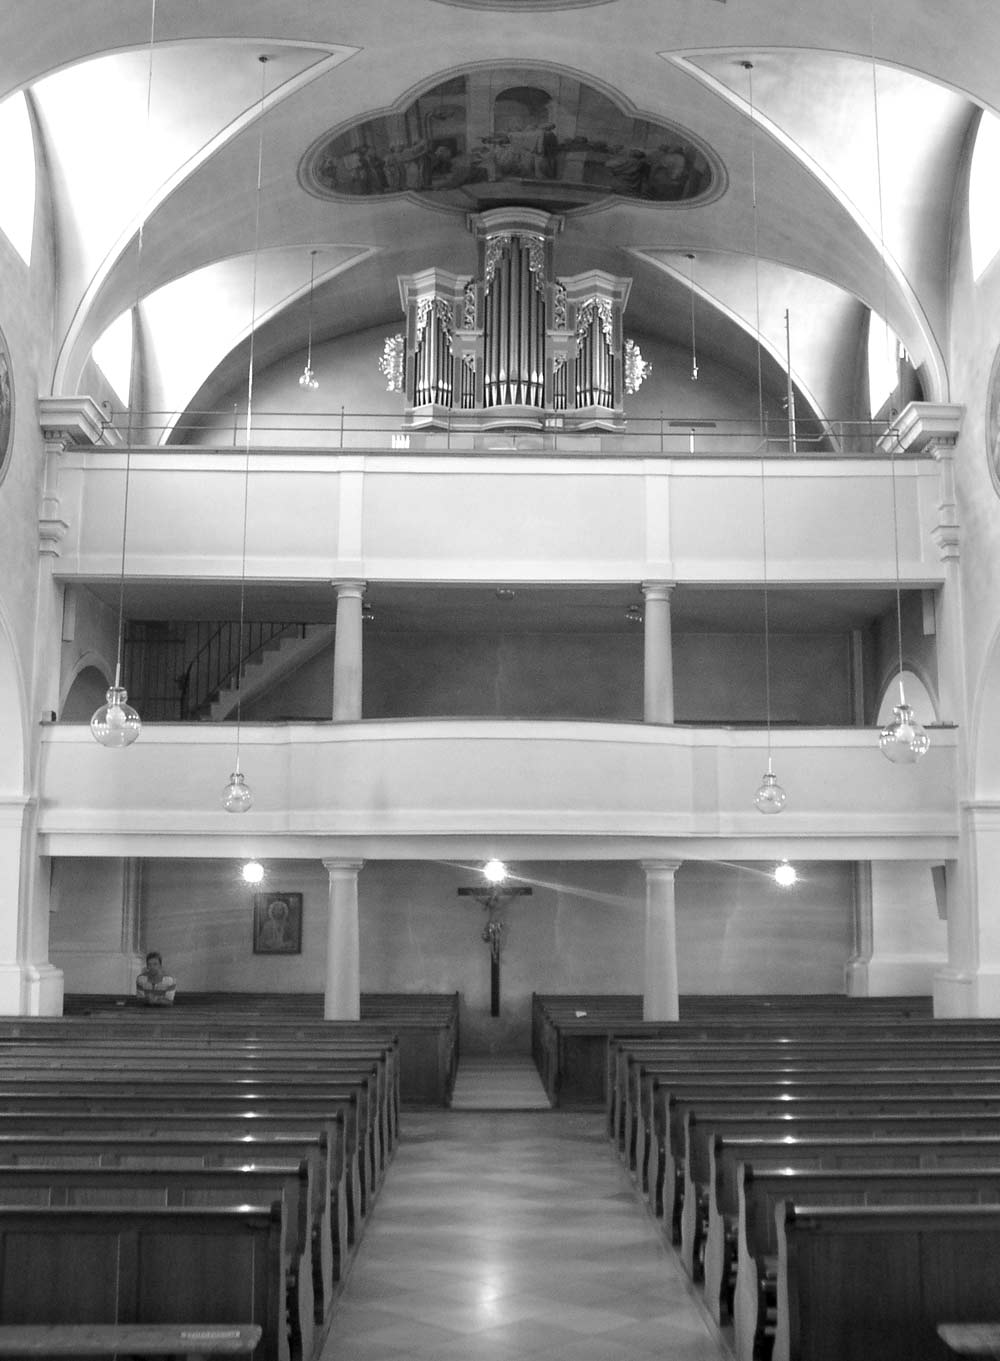
\includegraphics[width=5.001cm,height=6.805cm]{pictures/zulassungsarbeit-img037.jpg}

Pfarrkirche St. Laurentius
Ruhmannsfelden, Blick zur Orgelempore\\
\end{supertabular}
\end{flushleft}
\end{minipage}
\end{center}
Högns 3. Dienstzeit als Chorregent durchlief eine der schlimmsten Phasen
– nicht nur für die Kirchenmusik: Die Zeit des 2. Weltkriegs. Schon
1939 wurden vier Lehrer, die im Orchester mitwirkten,\footnote{
Interview Nr. 2, Barbara Essigmann, 27.12.2002, Absatz 4} zum
Kriegsdienst eingezogen. \footnote{Reicheneder-Chronik, Schulwesen,
Blatt 112 Vorder- und Rückseite} Einheimische Musiker des Orchesters,
wie Lorenz Schlagintweit, blieben von einem Kriegseinsatz genauso wenig
verschont. \footnote{Interview Nr. 13, Lorenz Schlagintweit,
29.11.2003, Absatz 2} Große Aufführungen mit Orchester an Festtagen,
wie von mehreren Zeitzeugen berichtet, \footnote{Interview Nr. 12,
Emilie Seidl, 23.4.2003, Absatz 14} dürften daher eher vor Ausbruch des
2. Weltkriegs, also zur Zeit von Chorregent Schroll, stattgefunden
haben. Besonders für das Streichorchester stellte der Krieg einen Bruch
dar. Als Ersatz etablierte sich eine Blechbläserformation, die sich aus
älteren Musikern der umliegenden Blaskapellen zusammensetzte. Die
Männerstimmen des Kirchenchores waren den Umständen entsprechend mit
nur zwei Sängern, nämlich Schwannberger und Holzfurtner, dünn
besetzt. \footnote{Interview Nr. 16, Maria Freisinger, 25.8.2004,
Absatz 6} Auch von der Orgel der Ruhmannsfeldener Pfarrkirche forderte
der Krieg seinen Tribut. Angesichts des geringen Metallgewinns, den die
am 12.6.1944 zum Ausbau bestimmten dünnwandigen Pfeifen und Leitungen
erbrachten, wird einerseits die aussichtslose Lage der
Kriegswirtschaft, andererseits die bewusste Schikane der Nazis
gegenüber der Kirche deutlich. Die Orgel – ihr fehlten die Register
Quintatön, Vox coelestis des ersten und alle metallischen Pfeifen
einschließlich der Windleitungen des zweiten Manuals\footnote{
Reicheneder-Chronik, Orgel, Blatt 74 Rückseite} – erlitt in der
Nachkriegszeit durch eine lange Trockenheit zusätzlichen großen
Schaden, ehe die Orgel 1947 vom Orgelbaumeister Kratochwill aus
Plattling restauriert wurde. \footnote{Högn, Ruhmannsfelden, S. 29}

Ob Högns Probenpraxis – die Proben fanden in seiner Wohnung
statt \footnote{Interview Nr. 2, Barbara Essigmann, 27.12.2002, Absatz
32} – eine Anpassung an den durch den Krieg geschmälerte Chor war oder
ob der Probenort auch schon in seiner ersten und zweiten
Chorregentenzeit derselbe war, kann aus Mangel an Zeitzeugen der
früheren Chorregentenzeiten nicht geklärt werden. Die Probenarbeit in
seiner Dienstwohnung hatte für Högn im allgemeinem einige praktische
Vorteile, und zwar aus folgenden Gründen: Hätte der Chor in der Kirche
geprobt, wäre es vor allem im Winter besonders kalt gewesen, da auf der
Orgelempore ein Fenster undicht war. \footnote{Interview Nr. 5, Barbara
Essigmann, 2.1.2003, Absatz 26} Einen beheizten Proberaum konnte die
Pfarrgemeinde damals nicht zu Verfügung stellen, sodass Högns große
Lehrerwohnung willkommene Alternative zur Kirche war. Außerdem besaß
Högn keinen Kirchenschlüssel, sodass er dem Mesner hätte Bescheid geben
müssen, damit die Kirche abends offen blieb. Nach der Probe hätte Högn
den Schlüssel im Pfarrhof zurückgeben müssen, was an sich relativ
umständlich gewesen wäre. \footnote{Interview Nr. 2, Barbara Essigmann,
27.12.2002, Absatz 88} Einige Zeitzeugen behaupten, dass nicht nur eine
einzige Stimmgruppe \footnote{Interview Nr. 2, Barbara Essigmann,
27.12.2002, Absatz 34} oder der komplette Chor in seiner Wohnung
probte, sondern auch das Blechbläserquartett. Nur die Generalprobe fand
in der Kirche statt. \footnote{Interview Nr. 13, Lorenz Schlagintweit,
29.11.2003, Absatz 4} Die Proben wurden auch nicht regelmäßig
abgehalten, beispielsweise jede Woche an einem bestimmten Wochentag,
sondern fanden nur dann statt, wenn ein neues Repertoire für große
Festtage erarbeitet werden musste. \footnote{Interview Nr. 2, Barbara
Essigmann, 27.12.2002, Absatz 48} Eine regelmäßige Probenarbeit machte
anscheinend wenig Sinn, wenn man sich den täglichen Einsatz der
Hauptsänger und –sängerinnen an den Gottesdiensten vergegenwärtig.
Durch die vielen Aufführungen hatte der Chor Routine und manche
Probearbeit wurde nach den Gottesdiensten geleistet.\footnote{
Interview Nr. 5, Barbara Essigmann, 2.1.2003, Absatz 36}

Vielleicht ist es aber auch auf die Proben in der privaten Wohnung
zurückzuführen, dass die Kirchenmusik in Ruhmannsfelden dem
deutschlandweiten Kulturaufschwung nach Ende des Krieges nicht folgte,
– man denke an die vielen Kleinkunstbühnen, die aus dem Boden schossen,
oder Konzerte, die in den Ruinen der ehemaligen Konzertsäle abgehalten
wurden – sondern eher einen Niedergang erlebte. \footnote{Interview Nr.
9, Dr. Doraliesa Wiegmann, 19.1.2003, Absatz 4; Interview Nr. 24,
Johann Glasschröder, 28.12.2004, Absatz 36} Die in Högns Wohnung
abgehaltenen Proben schienen zu einer Privatveranstaltung verkommen zu
sein. Nur für die Hauptsängerinnen hielt Högn Proben nach Ende des 2.
Weltkriegs. Die Sängerin Maria Freisinger hat jahrelang sonntags an den
Gottesdiensten mitgewirkt, doch an Proben konnte sie sich nicht
erinnern. \footnote{Interview Nr. 16, Maria Freisinger, 25.8.2004,
Absatz 8} Der öffentliche Chor wurde zu einem nach außen hin
abgeschlossenen Zirkel von eng befreundeten Hauptsängerinnen, zu dem
nur schwer neue Mitglieder stoßen konnten.

\begin{center}
\begin{minipage}{3.491cm}
\begin{flushleft}
\tablefirsthead{}
\tablehead{}
\tabletail{}
\tablelasttail{}
\begin{supertabular}{m{3.291cm}}

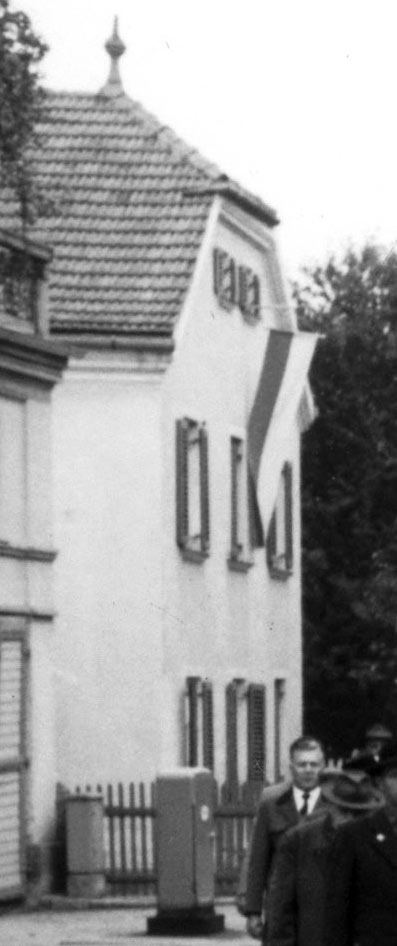
\includegraphics[width=3.108cm,height=7.408cm]{pictures/zulassungsarbeit-img038.jpg}

Im Erdgeschoss dieses Hauses wohnte
Högn ab 1945 bis zu seinem Tod\\
\end{supertabular}
\end{flushleft}
\end{minipage}
\end{center}
\begin{flushleft}
\tablefirsthead{}
\tablehead{}
\tabletail{}
\tablelasttail{}
\begin{supertabular}{m{4.6330004cm}}

\begin{center}

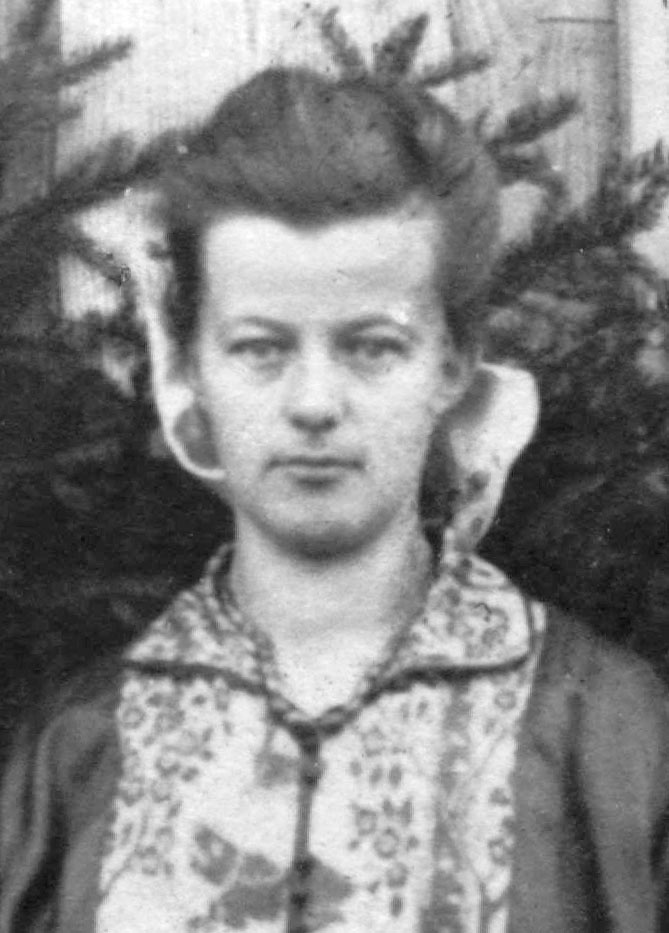
\includegraphics[width=4.3cm,height=5.973cm]{pictures/zulassungsarbeit-img039.jpg}

\end{center}
Theres Raster\\
\end{supertabular}
\end{flushleft}
Dass der Zustrom von neuen Sängerinnen und Sängern ausblieb, lag sicher
auch an dem Verhalten der Hauptsängerinnen. Sie hatten hauptsächlich
aus einem bestimmten Grund kein Interesse an einem größeren Chor:
Geld. \footnote{Interview Nr. 24, Johann Glasschröder, 28.12.2004,
Absatz 46} Denn je mehr Personen im Chor mitgesungen hätten, desto
öfter wäre die finanzielle Entschädigung, die dem Hauptchor zustand
aufzuteilen gewesen. Diese war etwa genau so hoch wie die des
Chorregenten. \footnote{Dokument Nr. 137, Chorabrechnung Ämter und
Messen, 3. Quartal 1952; Dokument Nr. 136, Chorabrechnung Beerdigungen
und Trauungen, 3. Quartal 1952; Dokument Nr. 138, Chorabrechnung, 4.
Quartal 1946} Das „Gehalt“ der einzelnen Sängerinnen wäre somit immer
kleiner ausgefallen. Aus dieser Sichtweise ist zum Beispiel das
Verhalten der Sängerin Theres Raster gegenüber neuen Chormitgliedern
durchaus nachvollziehbar. Raster war für den Notenschrank zuständig und
bestimmte sogar öfter als Högn, welches Stück gesungen werden
sollte. \footnote{Interview Nr. 2, Barbara Essigmann, 27.12.2002,
Absatz 94} Waren zu wenige Singstimmen vorhanden, und das war bei den
meist handgeschriebenen Notenmaterialien oft der Fall, gab sie
insbesondere den jungen Sängerinnen kein Notenblatt.\footnote{
Interview Nr. 16, Maria Freisinger, 25.8.2004, Absatz 8} Neue
Chormitglieder fühlten sich logischerweise weniger akzeptiert, wenn sie
wiederholt kein Notenblatt bekamen, noch dazu wenn ihnen nicht
klargemacht wurde, warum sie keine Stimmestimme bekommen
hatten. \footnote{Interview Nr. 16, Maria Freisinger, 25.8.2004, Absatz
12}

Der Hauptgrund, weshalb der Chor der Nachkriegszeit so wenige Mitglieder
zählte, ist aber in der Person von August Högn zu sehen. Mit 70 Jahren
hatte er nicht mehr den Elan, neue Sänger zu integrieren oder sich dem
intriganten Verhalten der Hauptsängerinnen entgegen zu
stellen. \footnote{Interview Nr. 16, Maria Freisinger, 25.8.2004,
Absatz 12} Vielleicht hat sich nicht nur sein hohes Alter, sondern auch
die Tatsache, dass er zeitlebens den Chorregentendienst nur
provisorisch oder aushilfsweise, paradoxerweise aber fast 20 Jahre lang
ausübte, wie in jedem Protokoll ausdrücklich erwähnt wird, und immer
nur als „Notnagel“ angesehen wurde, auf seine Einsatzbereitschaft
negativ ausgewirkt. Seinen drei großen heimatkundlichen Abhandlungen,
die alle in der Nachkriegszeit entstanden sind, entnimmt man, dass Högn
ab 1945 sein Hauptbetätigungsfeld nicht mehr in der Kirchenmusik sah.
